\chapter{Proposed Implementation}
\label{chap:impl}

My goal is to design and implement a library for \acrlong{acc:ea}, as mentioned in Chapter \ref{chap:intro}. The library should not only implement existing \acrshort{acc:ea} and allow to execute them on the \gpuns, but also afford a general framework to which it would be simple to plug new algorithms. For library users should be easy to replace evolutionary operators, modify them, or, if necessary, replace the whole workflow of the algorithm.

I decide to implement the library using Pipe and Filter architecture as specified by authors \citet{EnterpriseIntegrationPatterns}. The example of this architecture is in Figure \ref{fig:pipesandfilters}. The general idea is to partition the algorithm into smaller, simple steps and use the output of one step as the input to the following one. \acrshort{acc:ea} are simple to split as one step may be one evolutionary operator. I decided to implement the library in the \enquote{Convention over Configuration} design pattern -- that is, the operators make the same assumptions about the format and order of the input, rather than explicitly specifying it in the configuration. I still provide ways to control the order of parameters, if required by the user, and I will get to it a bit later.

\begin{figure}
    \centering
    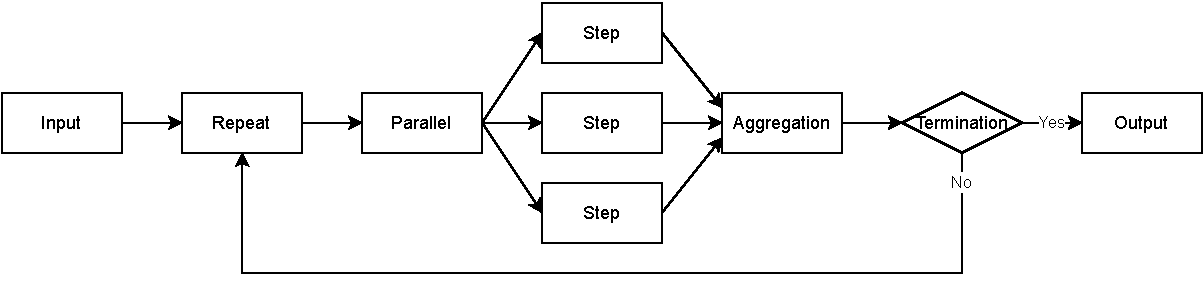
\includegraphics[width=\textwidth]{img/PipesAndFilters.pdf}
    \caption{Pipe and Filter architecture}
    \label{fig:pipesandfilters}
\end{figure}

The pure Pipe and Filter architecture is not sufficient for \acrshort{acc:ea} implementation. In the purest implementation, this architecture is just a chain of steps following each other. I decided to expand it by numerous practical steps like loops, parallel step invocation, and more. An example of parallel step and loop used in the Pipe and Filter architecture is demonstrated in Figure \ref{fig:pipesandfilters}. The parallel invocation is depicted in the figure by \enquote{Parallel} block, followed by the \enquote{Aggregation} block accumulating the results from each step. The loop is represented by the \enquote{Repeat} block accompanied by the \enquote{Termination} block controlling the loop termination condition.

My proposed implementation is the \emph{\acrlong{acc:ffeat}} (\acrshort{acc:ffeat}). This library is attached to this work, available on my GitHub \citep{FFEATrepo}, and ready for install as PyPI (Python Package Index) \href{https://pypi.org/project/FFEAT/}{package}. The PyPI is de facto standard way of installing Python packages from a central repository.

As I mentioned earlier, I decided to implement the library in the Python programming language and using PyTorch library. Python allows invocation of function with a variable number of arguments and a variable number of keyword arguments. Without explaining it in too much detail, arguments are passed into the function in a list and depend on their order. These are the traditional arguments known from languages like C and \cppns. Keyword arguments must be specified by their parameter name. The following line of code invokes function \textit{some\_function} with two parameters $1$ and $2$, and a keyword argument $karg=5$.

\begin{lstlisting}[language=Python]
some_function(1, 2, karg=5)
\end{lstlisting}

I use this design to implement operators in Pipe and Filter architecture. The operator accepts a variable number of normal and keyword arguments, and returns a list of variables and a dictionary. The list of variables and the dictionary serves as the input for the following operator as normal, respectively, as keyword arguments. Following this design, a new operator may be easily plug\-in into the algorithm. At the same time, it allows using the same underlying architecture both for genetic algorithms (the argument is only the population), as well as \acrshort{acc:pso} algorithms (using particles position, velocity, and their best--known positions as arguments).

The library expects the population to be represented as a tensor or as a list of tensors, where the first dimension enumerates over the individuals (note that the tensor needs to be aligned in each dimension). I resolve to this assumption because it allows me to implement the operators in vectorized manner and, therefore, more efficiently. Nevertheless, the architecture is general enough, and it may easily adjust to the problem at hand; the user would just need to reimplement the operators when necessary. In most cases, it is enough to represent the population using a single, two-dimensional tensor. Some operators are implemented in a way they may handle multidimensional tensors as well (for example the uniform crossover). In the case of \acrshort{acc:pso} algorithm, using a single tensor is not sufficient. The library represents the swarm using a list of tensors -- one tensor for each component of the population. Specifically, the library creates tensors for particles position and velocity, local and best--known positions, and their corresponding fitness values. Although the \acrshort{acc:pso} uses list of tensors, each of them still fulfills the requirement to use the first dimension to enumerate over individual particles. The operators can hence effectively run in parallel.

The library is split into several modules, focusing on different kinds of evolutionary algorithms or solving particular problems.
\begin{itemize}
    \item \incode{ffeat.flow} module includes basic classes to control the flow of the algorithm with the Pipe and Filter architecture in mind.
    \item \incode{ffeat.genetic} implements genetic algorithms operators and assume binary encoding.
    \item \incode{ffeat.strategies} contains all the real--\kern0.04em coded operators. Although not all of them are adaptive, therefore, they cannot be considered as evolution strategies, I decided to put them into the shared module for convenience.
    \item \incode{ffeat.pso} handles \acrlong{acc:pso} algorithms, their neighborhood and velocity update algorithms.
    \item \incode{ffeat.measure} implements aggregations functions focusing on fitness metrics.
    \item \incode{ffeat.utils} is a support module containing various useful functions like fitness scaling, decay, and early termination implementation.
\end{itemize}

The base class for all the operators is \incode{ffeat.Pipe}. The implementation merely accepts all the arguments and returns them. The specific logic needs to be provided by the derived class. The method the library invokes is the Python \incode{__call__} method allowing to call the object in the same way as if it was a function. That means the library invokes the operators using the standard invocation procedure, allowing the implementation of simple operators to be a function or a lambda function rather than a class.

The \incode{ffeat.flow} implements basal classes to use the Pipe and Filter architecture. I will refer to operators to invoke as \enquote{filters} to agree with the terminology used in the architecture. The most important filters are:
\begin{itemize}
    \item \incode{Sequence} executing filters in sequence and passing the output of the preceeding one into the following. The \incode{Sequence} class alone implements the simplest Pipe and Filter architecture.
    \item \incode{Parallel} executes filters in parallel -- that means all of them receive the same parameters, and their results are concatenated together. The execution is parallel from the logical point of view, not using multi threading.
    \item \incode{Repeat} executes filters in a loop for a given number of iterations (or indefinitely). The implementation allows breaking the loop early by passing \enquote{break} parameter as a keyword argument into the inner filters.
\end{itemize}
The module encompasses few more classes allowing to reorder and discard parameters (\incode{Select} class), replace some of them (\incode{Replace} class), transform each parameter (\incode{EachArg} class), and use Python lambda function (\incode{Lambda} class). I do not discuss them here, as the details are not important. Please see the attached source code for more information.

Before I describe particular operators, I would like to discuss the limitations of the PyTorch library and \gpu programming in general. As I already mentioned in Chapter \ref{chap:gpu}, the most costly situation is warp divergence. I tried to implement all the operators without condition statements and, therefore, eliminate the warp divergence situation as much as possible. I found boolean mask as a suitable replacement for condition statements. PyTorch may use boolean mask either for indexing (if the only portion of tensor should be updated) or in an arithmetic operation by multiplying tensor by the mask (and zeroing portion of the tensor).

A further limitation is the \gpu memory, which is a scarcer resource in comparison to the modern server machines. Modern graphical cards have up to low dozens of GB of memory (the latest NVIDIA V100 has 32GB of device memory \citep{nvidiav100spec}), whereas modern servers have hundreds of GB of memory. Because the library may use vast populations, even memory reallocation may be problematic, as the whole population must fit into the memory at least twice. I decided to implement the operators in--place, that is, all the operators are applied on the same memory. Not only it uses less memory, but it is also more efficient. Some operators (typically crossovers) have possibility to opt--out of in--place mode (for example, in the case of plus or comma crossover schema).

Operators using parents, for example crossovers and differential evolution, should receive distinct parents in order for the operator to do something useful. Unfortunately, this requirement is hard to satisfy, especially for \gpuns, because the parent indices are generated independently. It is, nevertheless, still possible using the \incode{torch.multinomial} function from the PyTorch library. The problem is that this function is very costly and its execution takes an order of magnitude more time than generating a random integer. I decided to allow specification of the parent sampling strategy for all these algorithms.



%%%%%%%%%%%%%%%%%%%%%%%%%%
%%                      %%
%%  GENETIC ALGORITHMS  %%
%%                      %%
%%%%%%%%%%%%%%%%%%%%%%%%%%
\section{Genetic Algorithms}
\label{chap:gaimpl}

The \acrlong{acc:ga} are in the \incode{ffeat.genetic} module. This module is further divided into the following submodules.
\begin{itemize}
    \item \incode{ffeat.genetic.initialization} holds classes initializing the population. I considered only random initialization and this is implemented by the \incode{Uniform} class.
    \item \incode{ffeat.genetic.evaluation} submodule contains classes to evaluate the individuals. The \incode{Evaluation} class expects to evaluate the whole population at once (ideal for \gpu implementation), whereas the \incode{RowEval} evaluates individuals one by one. Both classes expect to receive fitness function in their constructor.
    \item \incode{ffeat.genetic.mutation} includes mutation operators. The library only implements simple Bit--Flip mutation operator, allowing to specify a number of mutated individuals and the probability of gene change.
    \item \incode{ffeat.genetic.crossover} submodule.
    \item \incode{ffeat.genetic.selection} submodule.
\end{itemize}

I implemented uniform, one--point, and two--point crossovers for \acrshort{acc:ga} (classes \incode{Uniform}, \incode{OnePoint1D}, and \incode{TwoPoint1D}). The uniform crossover may handle individuals with an arbitrary number of dimensions because it simply generates a random mask of genes to inherit from the first parent. In the case of one-- and two--point crossovers the crossover point would be ambiguous; these, therefore, expect individuals to be one-dimensional. The one-- and two--point crossover implementation uses similar mask, but it is created based on the split point. That is a bit costly, especially for the two--point crossover, because each point must be added separately. The example implementation of one--point crossover is in Algorithm \ref{alg:implonepoint}.

All the crossover operators implement three distinct schemes of how to handle the offspring. The default scheme is the in--place version and the offspring replace their parents. For this to work, the crossover must produce the same number of offspring as there are parents. Moreover, the crossover operator should not process the whole population, as it may destroy it or shift the whole population into an undesirable region of the search space. Still, I decide to use it as the default version because of the \gpu limitations mentioned above.
The second and third schemes are the comma and plus schemes mentioned on Page \pageref{enum:steadystate}. The plus scheme concatenates the offspring with the parents and is specified by the \incode{replace_parents=False} argument. The comma scheme returns just the offspring and is specified by the \incode{discard_parents=True} argument passed to the crossover constructor.

\begin{algorithm}[b!]
\begin{lstlisting}[language=Python, xrightmargin=18pt]
import ffeat.genetic as GA


fn = create_problem_function()

alg = GA.GeneticAlgorithm(
    # Randomly initialize 100 individuals 
    # with gene of length 40
    GA.initialization.Uniform(100, 40),
    # Evaluate the population
    GA.evaluation.Evaluation(fn),
    # Sample 100 individuals into new generation
    GA.selection.Tournament(100),
    # Crossover 40% of them
    GA.crossover.OnePoint1D(0.4),
    # Mutate 60 of them with 1% mutation chance
    GA.mutation.FlipBit(60, mutate_prob=0.01),
    # repeat for 100 generations
    iterations=100
)
alg() # run the evolution
\end{lstlisting}
\caption{Simple \acrshort*{acc:ga} in \acrshort*{acc:ffeat}}
\label{alg:gaffeat}
\end{algorithm}

In the \incode{ffeat.genetic.selection} module the library keeps implementations of the 
tournament (\incode{Tournament} class)
roulette (\incode{Roulette} class), 
and \acrlong{acc:sus} (\incode{StochasticUniversalSampling} class)
selection operators. The tournament selection allows to specify whether is it maximization or minimization problem and a number of parents as I discussed in Chapter \ref{chap:eva}. Its implementation is in Algorithm \ref{alg:impltournament}. The rank--based selection operator is in fact the roulette or \acrshort{acc:sus} selection with fitness values preprocessing. I will get to fitness transformation later.

I also implemented elitism in the \incode{ffeat.genetic.selection.Elitism} class. It copies the $n$ best individuals from the population and temporarily stores them aside. After all the \acrshort{acc:ga} operators execute, it copies them back into the population. The implementation does not follow the exact description found in books \citep{IntroductionToEA}, because it may replace better individuals (when the elite improves). The standard implementations of elitism prohibit elites change by the following operators, or append the elites to the population after all the operators executed. 
Because the operators following the elitism may be arbitrarily complicated, or the user of the library may decide to implement their own set of operators, ensuring the elites would not change would be thorough and delicate work.
Moreover, from the \gpu programming point of view, copying a small amount of memory between an already allocated memory space is more efficient than appending the elites to the population, because that would require reallocation of the whole population. The implementation of the elitism operator is in Algorithm \ref{alg:implelitism}.

For convenience, the parameters dealing with population size, typically the number of individuals to sample during selection, or the number of offsprings in crossovers, can be specified using an absolute number or a fraction of the population size. Moreover, some operators parameters may change between the generations, for example mutation probability of Bit--Flip mutation. These parameters accept callable object evaluated each iteration, allowing them to adjust. Finally, there is no need to use \incode{ffeat.flow} module directly, but the flow is wrap in the \incode{ffeat.genetic.GeneticAlgorithm} class, into which the user just needs to plug the operators.

Example of a genetic algorithm in the \acrshort{acc:ffeat} library is in the Algorithm \ref{alg:gaffeat}.



%%%%%%%%%%%%%%%%%%%%%
%%                 %%
%%  REAL-CODED EA  %%
%%                 %%
%%%%%%%%%%%%%%%%%%%%%
\section{Real--Coded Evolutionary Algorithms}

Real--\kern0.04em coded evolutionary algorithms are encapsulated in the \incode{ffeat.strategies} module. It has a similar structure to \acrshort{acc:ga} module described above. Except for the operators mentioned above, I implemented operators specific to real--value encoding.

In the \incode{ffeat.strategies.crossover} submodule are uniform, one--point, and two--point crossovers identical to the ones for \acrshort{acc:ga}. Besides, it contains:
\begin{itemize}
    \item Arithmetic crossover in the \incode{Arithmetic} class. It allows specifying the number of parents and their weights. For $k$ parents, the offspring is created by the formula 
    $$\mathbf{o}_i=\sum_{j=1}^k w_{ji}\mathbf{p_j}_i$$
    It allows passing a callable object for the weights so that the weights may be randomized and the offspring may be different weighted arithmetic sum each generation (allowing different weights for genes as well).
    \item Blend crossover in the \incode{Blend} class, as described in the Chapter \ref{chap:eva}.
    \item Differential evolution implemented in the \incode{Differential} class. Although this operator may be used alone, I decided to keep it among the crossover operators. It is possible to alter the $F$ and $C$ constants over generations and replace the parent only if the offspring is better than its parent. In this case, the operator needs to know the fitness values of the parents.
\end{itemize}

\begin{algorithm}[b!]
\begin{lstlisting}[language=Python, xrightmargin=18pt]
import ffeat.strategies as ES


fn = create_problem_function()

alg = ES.EvolutionStrategy(
    # Randomly initialize 100 individuals 
    # in range (-5,5) with gene of length 40
    ES.initialization.Uniform(100, -5.0, 5.0, 40),
    # Evaluate the population
    ES.evaluation.Evaluation(fn),
    # Sample 100 individuals into new generation
    ES.selection.Roulette(100),
    # Crossover 40% of them
    ES.crossover.TwoPoint1D(0.4),
    # Use normal mutation for all of them with 
    # standard deviation 0.01
    ES.mutation.AddFromNormal(0.01),
    # repeat for 200 generations
    iterations=200
)
alg() # run the evolution
\end{lstlisting}
\caption{Simple real--\kern0.04em coded algorithm in \acrshort*{acc:ffeat}}
\label{alg:esffeat}
\end{algorithm}

From the mutation operators, I implemented the following operators in the \incode{ffeat.strategies.mutation} submodule.
\begin{itemize}
    \item Random replacement of gene by a value sampled from the specified distribution. It supports all the distributions implemented by the PyTorch library \citep{PyTorchDoc} and may refine the mutation rate over generations. It is implemented in the \incode{Replace} class, along with the \incode{ReplaceUniform} class sampling from uniform distribution.
    \item Small change of the individual by adding a value sampled from the specified distribution. It is encapsulated in the \incode{AddFromDistribution} class with specialized classes \incode{AddFromNormal} and \incode{AddFromCauchy} for normal and Cauchy distribution, respectively. The \incode{AddFromNormal} is the traditional implementation of normal mutation specified in the second chapter.
    \item Normal mutation with adaptive step implemented in the \incode{AdaptiveStep} class. It supports only the simplest adaptive algorithm by sharing the same deviation for all the dimensions. It allows specifying initial, maximal, and minimal deviation, as well as the step size and a number of better offspring needed to increase the deviation. This class may be used to implement the one--fifth rule.
\end{itemize}

The \incode{ffeat.strategy.EvolutionStrategy} class wraps together all the steps for real--\kern0.04em coded evolutionary algorithms. Simple real--\kern0.04em coded algorithm is in Algorithm \ref{alg:esffeat}.
    



%%%%%%%%%%%%%%%
%%           %%
%%  UTILITY  %%
%%           %%
%%%%%%%%%%%%%%%
\section{Utility functions}

I implemented some functionality allowing to control and measure the algorithm progress. The first set of these functions are in the \incode{ffeat.measure} module. It allows measuring statistical data like mean, deviation, and quantiles of the fitness. It passes measured metrics as keyword arguments to the following operator, so it is possible to stop the algorithm early if a specific metric does not improve or a certain threshold has been reached. Also, it is possible to log these metrics into standard output or file, if necessary.

The responsibility of the \incode{ffeat.utils.termination} submodule is the early termination of the algorithm. There are various termination criteria, for example if metric does not improve for a specified number of generations (\incode{NoImprovement} class), metric deviation for last $k$ steps is bellow a certain threshold (\incode{StdBellow} class), or metric reached the specified threshold (\incode{MetricReached} class).

The decay rates presented in Section \ref{chap:adaptiveoperators} are implemented in submodule \incode{ffeat.utils.decay} -- specifically the module implements linear, polynomial, and exponential decay rates. This module allows, for example, to decrease the mutation rate over generations.

The last submodule is \incode{ffeat.utils.scaling} which allows to rescale the fitness for the purposes of proportional--based selection operators. The fitness may be scaled linearly, exponentially, or using a logarithmic scale. The transformation of the minimization problem into the maximization one can be done using the \incode{MultiplicativeInverse} class that changes fitness using the $f(x)=1/x$ formula.

Earlier in this work, I have mentioned that rank--based selection operator is just a roulette-based selection operator with modified fitness values. The class \incode{RankScale} conducts that by sorting the population by the old fitness values and giving each individual a new fitness value based on its order. The given fitness values are linearly distributed among the population, but may be transformed into a different scale using one of the above--mentioned classes.




%%%%%%%%%%%%%%%%%%%%%%%%%%%%%%%%%%%
%%                               %%
%%  PARTICLE SWARM OPTIMIZATION  %%
%%                               %%
%%%%%%%%%%%%%%%%%%%%%%%%%%%%%%%%%%%
\section{Particle Swarm Optimization}

The \acrlong{acc:pso} algorithms are implemented in the \incode{ffeat.pso} module. It contains the implementation of both \acrshort{acc:spso2006} and \acrshort{acc:spso2011} algorithms, along the following neighborhoods in the \incode{ffeat.pso.neighborhood} submodule.
\begin{itemize}
    \item Random neighborhood.
    \item Nearest neighbors neighborhood.
    \item Static neighborhood is a helper class that caches the neighborhood in the first generation and uses it for the rest of the run. The following neighborhoods use the static neighborhood as their base class, and therefore the time to build the neighborhood does not affect the algorithm running time.
    \item Circle neighborhood with the possibility to specify the number of neighbors.
    \item Grid neighborhood with either linear, compact, or diamond shape, as specified in Chapter \ref{chap:psoneig}. The compact and diamond shapes are tricky to build in an arbitrary number of dimensions, so these are implemented only for two-dimensional cases and encapsulated in the \incode{Grid2D} class.
\end{itemize}

In the \incode{ffeat.pso.clip} submodule are classes allowing to clip either particles position or velocity. The whole \acrshort{acc:pso} algorithm is wraped inside the \incode{PSO} class. Because of the more complicated algorithm flow, this class does not allow as much freedom as previous \acrshort{acc:ga} or real--\kern0.04em coded \acrshort{acc:ea} implementations. The example of \acrshort{acc:pso} algorithm in \acrshort{acc:ffeat} is in Algorithm \ref{alg:psoffeat}.

\begin{algorithm}[b!]
\begin{lstlisting}[language=Python, xrightmargin=18pt]
import ffeat.pso as pso


fn = create_problem_function()

alg = pso.PSO(
    # Randomly initialize position of 100 particles
    pso.initialization.Uniform(100, -5.0, 5.0, 40),
    # Randomly initialize velocities
    pso.initialization.Uniform(100, -1.0, 1.0, 40),
    # Pass the evaluation function
    pso.evaluation.Evaluation(fn),
    # Specify random neighborhood with 3 neighbors
    pso.neighborhood.Random(3),
    # Use SPSO2006 velocity update rule
    pso.update.PSO2006(
        inertia=0.8, 
        local_c=1.5, 
        global_c=1.5
    ),
    # Clip particles position into range
    clip_position=pso.clip.Position(-5,5),
    # Clip particles velocity
    clip_velocity=pso.clip.VelocityNorm(2.0),
    # Specify number of iterations
    iterations=200
)
alg() # run the PSO algorithm
\end{lstlisting}
\caption{\acrshort*{acc:pso} algorithm in \acrshort*{acc:ffeat}}
\label{alg:psoffeat}
\end{algorithm}
